\documentclass[12pt]{article}
\usepackage{graphicx} % Required for inserting images
\usepackage{geometry}
\usepackage{amsmath}
\usepackage{hyperref}
\usepackage{amsmath}
\usepackage{enumitem}
\usepackage{amsfonts}
\usepackage{amssymb}
\usepackage{graphicx}
\usepackage{hyperref}
\usepackage{listings}
\usepackage{xcolor}
\usepackage{titling}
\usepackage{amsmath}
\usepackage{amssymb}
\usepackage{listings}
\usepackage{url}
\usepackage{tikz}

\lstset{
  basicstyle=\ttfamily\small,
  breaklines=true,
  frame=single,
  numbers=left,
  numberstyle=\tiny,
  keywordstyle=\bfseries\color{blue}
}

\lstdefinestyle{cuda}{
    language=C++,
    basicstyle=\ttfamily\footnotesize,
    keywordstyle=\color{blue},
    commentstyle=\color{gray},
    stringstyle=\color{red},
    numbers=left,
    numberstyle=\tiny,
    stepnumber=1,
    breaklines=true,
    tabsize=4
}

\begin{document}

% Include the title page
\title{Schur Numbers Week 6 Report}
\date{\today}
\begin{titlepage}
    \begin{center}
        \vspace*{1cm}

        \rule{\linewidth}{0.2mm} \\[0.4cm]
        {\Large \textbf{CSE 326 Analysis and Design of Algorithms }}\\[0.4cm]
        \textbf{Dr.Walid Gomaa}
 
        \rule{\linewidth}{0.2mm} \\[1.5cm]

        \begin{tabular}{c}
            \begin{tabular}{ll}
                \textbf{Name} & \textbf{ID} \\
                \hline
                Mohamed Abdelmonem Makram & 120220055 \\
                \hline
                Abdelrahman Ahmed Shaheen & 120220228 \\
                \hline
                Abdelrhman Mohamed Eldenary & 120220253 \\
                \hline
                Anas Ihab  Badr & 120220360 \\
                

            \end{tabular}
        \end{tabular}

        \vspace{1cm}

        

        \vspace{5cm}

        
\includegraphics[width=0.25\textwidth]{ejust.jpg}


        Computer Science Engineering Department\\
        Egypt-Japan University of Science and Technology\\

    \end{center}
\end{titlepage}


\tableofcontents
\newpage
\maketitle
\section{Introduction}
This week our work was divided into 3 main parts. First part is that we would explore the Schur numbers
problem as a SAT (Satisfiability) problem. Second part is summarizing past papers on CUDA programming 
in solving NP problems (Schur numbres is stated to be a near NP problem). Third part is actually getting 
CUDA code to run on our machines (not very straight forward). In this report we will explain
each of these parts in detail, hopefully.



\section{SAT Approach in Schur Number Problem}

In this week’s report, we explored the SAT-based methods used to address the Schur number problem. Building on our previous findings, where we stated, \textit{“We would go back to understand the SOTA paper on how they developed Schur number 5”}, we have now analyzed the SAT-solving approach in depth. Below, we summarize our findings.

\subsection{How SAT Solvers Work}
SAT solvers are tools designed to determine the satisfiability of a propositional logic formula in Conjunctive Normal Form (CNF). For the Schur number problem, the goal is to encode the coloring constraints into a propositional formula and verify if a valid coloring exists for a given number of colors and integers.


In the implementation, Z3 library was used, a high-performance theorem prover and SAT solver. Z3 provides a Python API, which allowed us to efficiently encode constraints, solve problems, and analyze results. The entire implementation, including the code discussed in this report, is available in our GitHub repository. This implementation facilitated the generation of CNF formulas, applying constraints, and optimizing the search space.


\subsection{Constraints Used in the SAT Encoding}
To ensure the encoding correctly represents the problem, several key constraints are applied:

\begin{enumerate}
    \item \textbf{Each number must have exactly one color:}
    Each integer \( j \) (\( 1 \leq j \leq n \)) is assigned one and only one color among \( k \) colors. This constraint is encoded as:
    \[
    \bigvee_{i=1}^{k} v_{ij}
    \]
    \[
    \neg(v_{i1} \land v_{i2} \land \ldots \land v_{ik})
    \]
    The equivalent Python code is:
    \begin{lstlisting}[language=Python]
    # At least one color
    s.add(Or(colors[i]))
    # At most one color
    s.add(Not(And(colors[i])))
    \end{lstlisting}

    \item \textbf{No monochromatic solution to \( a + b = c \):}
    For any triple \( (a, b, c) \) satisfying \( a + b = c \), the numbers \( a \), \( b \), and \( c \) cannot all have the same color. This is expressed as:
    \[
    \neg(v_{ia} \land v_{ib} \land v_{ic}), \forall i \in [1, k]
    \]
    The equivalent Python code is:
    \begin{lstlisting}[language=Python]
    for a in range(1, n+1):
        for b in range(a, n+1):
            c = a + b
            if c <= n:
                for i in range(k):
                    s.add(Not(And(colors[a-1][i], colors[b-1][i], colors[c-1][i])))
    \end{lstlisting}

    \item \textbf{Symmetry breaking:}
    To reduce redundant searches caused by color permutation, additional constraints are imposed, such as assigning specific colors to initial numbers. For example:
    \[
    v_{11} = 1, \quad v_{22} = 1
    \]
    The equivalent Python code is:
    \begin{lstlisting}[language=Python]
    s.add(colors[1-1][0]) # Assign color 0 to number 1
    s.add(colors[2-1][1]) # Assign color 1 to number 2
    \end{lstlisting}

    \item \textbf{Additional heuristics:}
    Custom heuristics prevent invalid patterns, such as two consecutive numbers having the same color:
    \[
    \neg(v_{i1} \land v_{i2}), \quad \forall i \in [1, k]
    \]
    Similarly, for preventing overlap in specific patterns:
    \[
    \neg(v_{i1} \land v_{i3}), \quad \forall i \in [1, k]
    \]
    The equivalent Python code is:
    \begin{lstlisting}[language=Python]
    for i in range(n-1):
        s.add(Not(And(colors[i][0], colors[i+1][0])))
    # Prevent overlap in specific patterns
    for i in range(n-2):
        s.add(Not(And(colors[i][1], colors[i+2][1])))
    \end{lstlisting}
\end{enumerate}

The constraints work together as follows:
\begin{itemize}
    \item \textbf{Organizing the search space:} Constraints (1) ensure each number has one and only one color.
    \item \textbf{Avoiding conflicts:} Constraint (2) prevents any monochromatic solution to \( a + b = c \), ensuring the validity of the coloring.
    \item \textbf{Speeding up the computation:} Constraint (3) reduces the search space by breaking symmetries, and Constraint (4) introduces additional optimizations for efficient solving.
\end{itemize}

\subsection{Cube-and-Conquer Method}
The Cube-and-Conquer (C\&C) method enhances SAT solvers by splitting the problem into smaller subproblems ("cubes") that can be solved independently. This method consists of two phases:
\begin{enumerate}
    \item \textbf{Cube Phase:} The problem is divided into millions or billions of smaller subproblems using decision heuristics. Each subproblem represents a partial assignment of variables.
    \item \textbf{Conquer Phase:} Each subproblem (cube) is solved using a Conflict-Driven Clause Learning (CDCL) solver. Solutions from these subproblems are combined to form the final result.
\end{enumerate}

This hybrid approach combines the strengths of look-ahead solvers for splitting and CDCL solvers for solving, enabling efficient parallel processing.

\subsection{Proofs Used in the Paper}
Three main types of proofs to ensure correctness and completeness were developed and verified: 
\begin{enumerate}
    \item \textbf{Re-encoding Proof:} This proof validated the correctness of the symmetry-breaking techniques used to reduce the search space. It ensured that the modified formulas preserved the logical equivalence of the original problem.

    \item \textbf{Implication Proof:} This proof demonstrated that \( S(5) > 160 \) is unsatisfiable by partitioning the problem into smaller cubes and proving unsatisfiability for each subproblem. The total size of this proof exceeded two petabytes.

    \item \textbf{Tautology Proof:} This proof confirmed that the cubes covered the entire search space, ensuring that no valid solution was overlooked.
\end{enumerate}
These proofs were validated using the ACL2 theorem prover, providing high confidence in the correctness of the results.

\subsection{Results of the SAT Approach and Cube-and-Conquer}
The SAT-based Cube-and-Conquer method produced the following results:
\begin{itemize}
    \item Confirmed that \( S(5) = 160 \).
    \item Partitioned the search space into over 10 million subproblems, solved efficiently in parallel.
    \item Generated a proof of unsatisfiability for \( S(5) > 160 \), with a total proof size exceeding two petabytes.
    \item Achieved a runtime of just three days on a high-performance computing cluster (equivalent to 14 CPU years).
\end{itemize}

These findings highlight the power and scalability of the SAT-based Cube-and-Conquer method in addressing complex combinatorial problems like the Schur number problem.


\section{Running CUDA Code on Local Machines}
We managed to run CUDA code on one of our machines. The coding part 
was the easiest but setting up the environment was the hardest. LLMs cannot really do that
for you. The code though was generated using an LLM for our basic two-pointers approach. However,
we are sure that they are not perfect in making efficient, memory optimized code so our goal in the
next week to improve more on the code and explore replicating the results of "Schur Number Five" paper, hopefully.
The code is available in \texttt{code/Cuda code} directory in our repository. The reason it has an inconvenient name is because we 
used a sample code from their official website and modified the content only. We're still exploring how to 
build the code ourselves. The results of the code were promising as shown in the image below. which compared to the previous threading approach 
in the last week this is 3x faster. 50 ms vs 150 ms.
\begin{figure}[h]
    \centering
    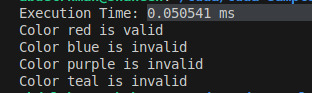
\includegraphics[width=0.8\textwidth]{results.jpg}
    \caption{Results of running the CUDA code}
    \label{fig:results}
\end{figure}
\\ \\
\textbf{LLM Prompt:}
\textit{
\\
\texttt{>>} Do you Schur numbers problem? \\
\texttt{<<} *Some explanation from the LLM* \\
\texttt{>>} I need you start with the following coloring
{"red", {1, 4, 9, 12, 19, 26, 33, 36, 41}},
{"blue", {2, 3, 10, 11, 16, 29, 30, 34, 35, 42, 43}},
{"purple", {5, 6, 7, 8, 17, 18, 27, 28, 37, 38, 39, 40}},
{"teal", {13, 14, 15, 20, 21, 22, 23, 24, 25, 31, 32}},
Then i want you to spawn 5 threads. Each thread will take a color and do 2 pointer algorithm where we initialize L and R pointers to the start and end of each array. we want to see which colors can we add the next number to which is 44. The pointers will iterate to sum the values pointed by L and R, if it's bigger than the number to add (44) we decrement R, if it's less than the number we increment L. If we found a solution then this color is not valid. If we don't then this color is valid. After the execution i want the program to output the execution time and what is the new colorings.}



\section{Past Papers on CUDA Programming in NP Problems}

We reviewed three papers from the recent literature that discuss the use of CUDA programming in solving NP problems. The papers are as follows:

\subsection{CUDA-NP: Nested Parallelism in GPGPU Applications}
CUDA-NP is a framework designed to enhance nested thread-level parallelism (TLP) in CUDA applications. Traditional dynamic parallelism suffers from kernel launch overhead and global memory bottlenecks. CUDA-NP improves execution by:
\begin{itemize}
    \item Remapping threads into a 1D structure for better execution control.
    \item Assigning multiple slave threads to master threads to handle nested loops in parallel.
    \item Utilizing registers and shared memory to reduce memory latency.
\end{itemize}

Performance benchmarks on NVIDIA GTX 680 GPUs demonstrated up to a 6.69× speedup compared to baseline implementations, with an average improvement of 2.01×. This method is particularly effective for workloads containing nested loops, such as dynamic programming problems and graph-based algorithms.

\subsubsection{Our Takeaways}
CUDA-NP effectively addresses the inefficiencies of dynamic parallelism by restructuring execution models. Its use of hierarchical memory and optimized thread execution significantly reduces computation overhead in nested parallel workloads.

\subsection{Nested Parallelism in GPGPU Programs}

Nested parallelism is crucial for GPGPU applications that rely on thread-level parallelism to mask memory latencies. One illustrative example is the Transposed-Matrix-Vector Multiplication (TMV), where each GPU thread computes an element of the output vector. The kernel implementation ensures efficient memory access by distributing computations across multiple threads, significantly reducing execution time.

The proposed optimization focuses on:
\begin{itemize}
    \item Restructuring kernels to leverage hierarchical memory.
    \item Using thread indexing efficiently to maximize parallel execution.
    \item Avoiding redundant memory accesses to optimize performance.
\end{itemize}

These improvements directly impact graph processing and combinatorial optimization problems, where large-scale matrix computations are frequently involved.

\subsubsection{Our Takeaways}
This approach highlights the importance of hierarchical execution structures and optimized memory access in enhancing CUDA performance, particularly for matrix computations and large-scale data operations.

\subsection{CUDA-NP: A Directive-Based Compiler Framework for Nested Parallelism}

CUDA-NP extends its optimization approach using compiler directives similar to OpenMP. The framework automatically transforms CUDA kernels by:
\begin{itemize}
    \item Modifying thread hierarchies to introduce slave threads.
    \item Adjusting control flow to enable parallel execution within loops.
    \item Enhancing memory usage by prioritizing shared memory over global memory.
    \item Distributing workload across multiple threads, reducing overall execution time.
\end{itemize}

The directive-based approach simplifies the optimization process, making it easier to integrate nested parallelism into existing CUDA applications.

\subsubsection{Our Takeaways}
Directive-based transformations provide an efficient way to integrate nested parallelism in CUDA programs, automating optimizations that would otherwise require extensive manual intervention.

\subsection{Application to Schur Numbers Problem}

The Schur Numbers problem, an NP-hard problem in combinatorial number theory, involves partitioning sets of integers while avoiding monochromatic solutions under specific constraints. CUDA's parallelization capabilities can significantly enhance brute-force and heuristic search approaches for finding new Schur numbers.

Applying the techniques from the reviewed papers to Schur Numbers involves:
\begin{itemize}
    \item Implementing nested parallelism for evaluating partitions concurrently.
    \item Using optimized memory management techniques to store intermediate results efficiently.
    \item Reducing thread divergence by leveraging hierarchical execution strategies.
\end{itemize}

By integrating CUDA-NP's compiler optimizations, execution speed can be enhanced, making the exploration of larger Schur numbers feasible.


\section*{References}
Heule, M. J. H. (2017). \textit{Schur Number Five}. arXiv. https://arxiv.org/abs/1711.08076

\end{document}